\chapter{Расчет параметров выпрямительной установки возбуждения (ВУВ)}
\section{Определение эксплуатационных характеристик ВУВ}

В качестве ВУВ используем однофазный управляемый двуполупериодный выпрямитель, выполненный по мостовой схеме. При сборе схемы электродинамического торможения, обмотки возбуждения всех тяговых двигателей секции электровоза соединяются последовательно и подключаются к выходу ВУВ. 

Расчетная схема силовой части ВУВ изображена на рисунке~\ref{fig:vuv}.

\begin{figure}[H]
    \centering    
    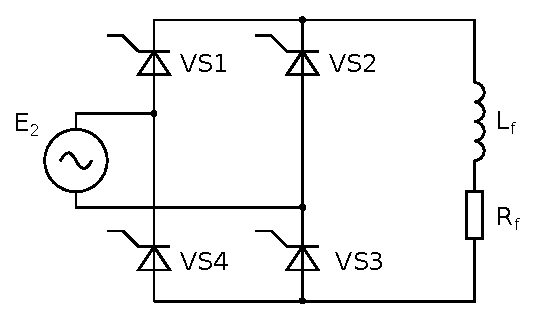
\includegraphics[width=0.5\textheight]{rectifier.eps}
    \caption{Расчетная схема силовой части выпрямительной установки возбуждения: $E_2$ - ЭДС обмотки тягового трансформатора, выделенной для питания ВУВ; VS1~--~VS4 - однооперационные тиристорные ключи; $L_f, \, R_f$ - соответственно, эквивалентная индуктивность и эквивалентное активное сопротивление обмоток возбуждения ТЭД.}
    \label{fig:vuv}
\end{figure}

Нагрузка выпрямительной установки носит активно-индуктивный характер. Ток, протекающий через нагрузку $I_d$ определяется исходя из результата расчетов, приведенных в таблице~\ref{tab:I_field_reg}. Принимаем его $I_d = 857$ А. Максимальное напряжение на зажимах ВУВ расчитываем исходя из эквивалентного сопротивления шести последовательно соединенных обмоток возбуждения

\begin{equation*}
 R_{f} = n_a \, R_{\text{в}} = 6 \cdot 0,03 = 0,18 \, \text{Ом}
\end{equation*}
исходя из чего, по данным таблицы~\ref{tab:I_field_reg}, определяем диапазон регулирования выходного напряжения
\begin{equation*}
 U_d^{\min} = 200 \cdot 0,18 = 36, \, \text{В} \quad U_d^{\max} = 857 \cdot 0,18 = 155, \, \text{В}
\end{equation*}

При минимальном угле открытия тиристоров $\alpha_0 = 9^\circ$ (обеспечивающем надежное их открытие) и с учетом работы на индуктивную нагрузку, расчитаем максимальное среднее значение напряжение на выходе ВУВ
\begin{equation*}
 U_0 = \frac{U_d^{\max}}{\cos \, \alpha_0} = \frac{155}{\cos \, 9^{\circ}} = 157, \, \text{В}
\end{equation*}
Рассчитываем угол открытия тиристоров при минимальном напряжении на выходе ВУВ
\begin{equation}
 \alpha_{\max} = \arccos \left( \frac{U_d^{\min}}{U_0} \right) = \arccos \left( \frac{36}{157} \right) = 76^{\circ}
\end{equation}

Определяем максимальное обратное напряжение на тиристоре, для схемы мостового выпрямителя
\begin{equation*}
 U_{VS}^{\max} = 3,14 \, U_0 = 3,14 \cdot 157 = 493, \, \text{В}
\end{equation*}
Расчетное значение повторяющегося напряжения на тиристоре
\begin{equation*}
 U_{\text{пр}} = k_{U} \, k_{\text{с}} \, U_{VS}^{\max} 
\end{equation*}
где $k_{U} = 1,3 \div 1,5$ - коэффициент запаса по напряжению; $k_{\text{с}} = 1,16$ - коэффициент, учитывающий возможное повышение напряжения в контактной сети до предельного значения 29 кВ, то есть, в нашем случае
\begin{equation*}
 U_{\text{пр}} = 1,4 \cdot 1,16 \cdot 493 = 800, \, \text{В} 
\end{equation*}

Расчетное значение предельного тока тиристора определяем по формуле
\begin{equation*}
 I_{\text{пр}} = k_I \, k_{\text{ф}} \, k_{\text{охл}} \, I_d
\end{equation*}
где $k_I = 1,25 \div 1,4$ - коэффициент запаса по току; $k_{\text{ф}} = 0,9$ - коэффициент формы тока, учитывающий его несинусоидальность; $k_{\text{охл}}$ - коэффициент, учитывающий условия охлаждения тиристоров ($k_{\text{охл}}$ = 2,5 - при стандартном радиаторе без обдува; $k_{\text{охл}} = 1,0$ - при принудительном воздушном охлаждении. Тогда, в нашем случае

\begin{equation*}
 I_{\text{пр}} = 1,25 \cdot 0,9 \cdot 1,0 \cdot 857 = 964 \approx 1000, \, \text{А}
\end{equation*}

Тиристор выбираем из условия 
\begin{equation*}
 U_{\text{п}} \ge U_{\text{пр}}, \quad I_{\text{п}} \ge I_{\text{пр}}
\end{equation*}
где $U_{\text{п}}$ - максимально допустимое мгновенное напряжение, прикладываемое к тиристору; $I_{\text{п}}$ - предельное значение тока тиристора.

Указанным условиям удовлетворяет тиристор  марки T133-500 производства ПАО <<Электровыпрямитель>> (г.~Саранск).

Тиристор Т133-500 имеет исполнение таблеточного типа в корпусе PT31. Технические характеристики тиристора указаны в нижеприведенной таблице

\begin{figure}[H]
    \centering        
    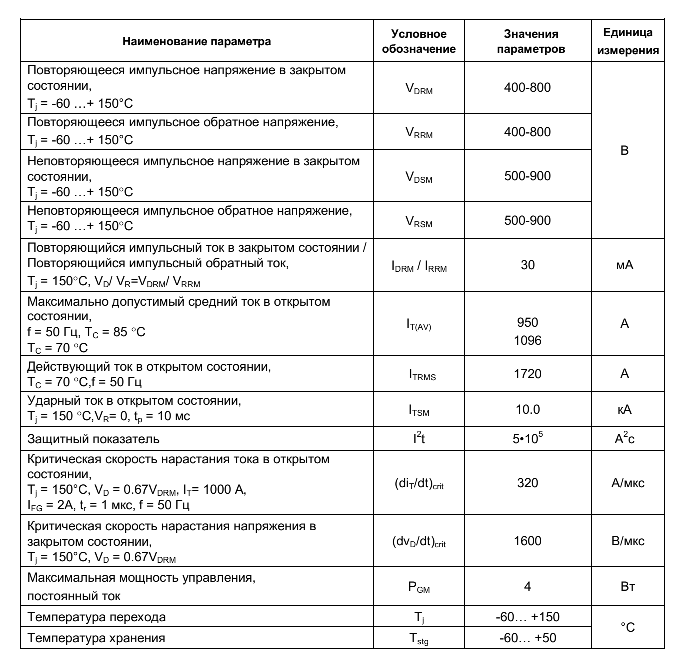
\includegraphics[width=0.6\textheight]{T133-500.eps}    
    \label{fig:T133-500}
\end{figure}

\section{Определение параметров обмотки тягового трансформатора, питающей ВУВ}

Рассчитываем действующее значение напряжения на вторичной обмотке тягового трансформатора
\begin{equation*}
 U_2 = \frac{\pi \, U_0}{2\,\sqrt{2}} = \frac{3,14 \cdot 157}{2\,\sqrt{2}} = 174, \, \text{В} 
\end{equation*}
Принимая КПД трансформатора равным 95\%, расчитываем габаритную мощность обмотки
\begin{equation*}
 S_2 = \frac{U_2 \, I_d}{1000 \, \eta}  = \frac{174 \cdot 857}{1000 \cdot 0,95} \approx 158, \, \text{кВт}
\end{equation*}

Определяем мощность потерь в обмотке
\begin{equation*}
 \Delta \, P_2 = S \, (1 - \eta) = 158 \cdot (1 - 0,95) = 7,9, \, \text{кВт}.
\end{equation*}
Полагая, что 50\% потерь рассеиваются в меди, рассчитываем величину активного сопротивления обмотки
\begin{equation*}
 r_2 = \frac{500 \, \Delta P_2}{I_d^2} = \frac{500 \cdot 7,9}{857^2} = 0,0054, \, \text{Ом}
\end{equation*}

\section{Расчет нагрузочной характеристики выпрямительной установки}

Нагрузочной характеристикой ВУ называется зависимость напряжения на нагрузке от тока, протекающего через него. Для управляемого выпрямителя она имеет вид
\begin{equation}
 \label{eq:out_char}
 U(I) = U_{\text{хх}} - (r_2 + 2 \, r_{\text{т}}) \, I
\end{equation}
где $U_{\text{хх}}$ - напряжение холостого хода при постоянном угле открытия тиристоров; $r_2$ - сопротивление вторичной обмотки трансформатора; $r{\text{т}}$ - сопротивление тиристора в открытом состоянии. Для тиристора Т133-500 $r{\text{т}} = 0,00042$ Ом. Из формулы \eqref{eq:out_char} выражаем значение напряжения холостого хода
\begin{equation}
 \label{eq:Uxx}
 U_{\text{хх}} = U_d + (r_2 + 2 \, r_{\text{т}}) \, I_d
\end{equation}
Из формулы \eqref{eq:Uxx} находим напряжение холостого хода при минимальном и максимальном значении напряжения на нагрузке
\begin{equation}
\label{eq:Uxxmin}
 U_{\text{хх}}^{\min}(76^{\circ}) = U_d^{\min} + (r_2 + 2 \, r_{\text{т}}) \, I_d^{\min} = 36 + (0,0054 + 2 \cdot 0,00042) \cdot 200 = 37, \text{В}
\end{equation}
\begin{equation}
\label{eq:Uxxmax}
 U_{\text{хх}}^{\max}(9^{\circ}) = U_d^{\max} + (r_2 + 2 \, r_{\text{т}}) \, I_d^{\max} = 155 + (0,0054 + 2 \cdot 0,00042) \cdot 857 = 160, \text{В}
\end{equation}
Подставляем \eqref{eq:Uxxmin} и \eqref{eq:Uxxmax} в \eqref{eq:out_char}, получая выходные характеристики ВУВ при минимальном и максимальном угле открытия тиристоров
\begin{align}
 \label{eq:min_deg}
 & U_{9^{\circ}}(I) = 160 - 0,0064 \, I \\
 \label{eq:max_deg}
 & U_{76^{\circ}}(I) = 37 - 0,0064 \, I 
\end{align}
По формулам \eqref{eq:min_deg} и \eqref{eq:max_deg} вычисляем  значения напряжения на выходе ВУВ для нескольких значений тока вобуждения, сводя результаты в таблицу~\ref{tab:out_char} 

\begin{table}[H]
 \centering
 \caption{Нагрузочная характеристика выпрямительной установки возбуждения}
 \begin{tabular}{|c|c|c|c|c|c|c|c|c|c|c|}
  \hline
  I, А & 0 & 100 & 200 & 300 & 400 & 500 & 600 & 700 & 800 & 900 \\ \hline
  $U_{9^{\circ}}$ & 160,0 & 159,4  & 158,7 & 158,1 & 157,5 & 156,9 & 156,3 & 155,6 & 155,0 & 154,4\\ \hline
  $U_{76^{\circ}}$ & 37,0 & 36,4 & 35,8 & 35,1 & 34,5 & 33,9 & 33,3 & 32,6 & 32,0 & 31,8  \\ \hline
 \end{tabular}
 \label{tab:out_char}
\end{table}

По данным таблицы~\ref{tab:out_char} строим график нагрузочной характеристики ВУВ (рисунок~\ref{fig:out_char_vuv})
\begin{figure}[H]
    \centering    
    \includegraphics[width=0.5\textheight]{out_char_vuv.eps}
    \caption{Нагрузочные характеристики ВУВ при предельных углах открытия тиристоров}
    \label{fig:out_char_vuv}
\end{figure}










